\documentclass[11pt,pdftex]{article}

\usepackage{amsmath}
\usepackage{amsfonts}
\usepackage{graphicx}
\usepackage{url}
\usepackage{cite}
\usepackage{algorithm,algorithmic}
\usepackage{color}
\usepackage{times}
\usepackage{bm}
\usepackage{a4}
\usepackage{url}
\usepackage{hyperref}
\usepackage{tikz}
\usepackage{pgflibraryshapes}  
\usetikzlibrary{arrows}
\usetikzlibrary{mindmap,trees}
\usepackage[overlay,absolute]{textpos}
\usepackage{pgfpages}

\newcommand{\opal}{\textsc{OPAL}}
\newcommand{\opalt}{\textsc{OPAL-t }}
\newcommand{\opale}{\textsc{OPAL-e }}
\newcommand{\opalcycl}{\textsc{OPAL-cycl}}
\newcommand{\opalmap}{\textsc{OPAL-map }}
\newcommand{\opalenv}{\textsc{OPAL-envelop}}

\newcommand{\mad}{\textsc{mad }}
\newcommand{\madnine}{\textsc{mad9 }}
\newcommand{\madninep}{\textsc{mad9p }}
\newcommand{\madeight}{\textsc{mad8 }}

\newcommand{\classic}{\textsc{classic }}
\newcommand{\hfifepart}{\textsc{H5Part }}
\newcommand{\hfifefe}{\textsc{H5FED }}

\renewcommand{\epsilon}{\varepsilon} 
\renewcommand{\vec}[1]{{\bf #1}} 
\newcommand{\dt}[1]{\frac{\partial #1}{\partial t}}
\newcommand{\dtt}[1]{\frac{\partial^2 #1}{\partial t^2}}
\newcommand{\dtvec}[1]{\frac{\partial {\mathbf #1}}{\partial t}}
\newcommand{\dttvec}[1]{\frac{\partial^2 {\mathbf #1}}{\partial t^2}}
\newcommand{\rot}{\vec{\nabla} \wedge }
\renewcommand{\div}{\vec{\nabla} \cdot }

\def\vec#1{\mathbf{#1}}
\def\vecg#1{\boldsymbol{#1}}
\def\norm#1{\| #1 \|} 
\def\tr{^{\!\top}}

\def\curl{{\bf curl}\,}
\def\curlp{{\rm curl}_p\,}
\def\div{{\rm div}\,}
\def\grad{\nabla}
\def\gradp{\nabla_p}
\def\dotp#1#2{\langle#1,#2\rangle}
\def\eps{\varepsilon}

\newcommand{\mat}[1]{\ensuremath{\boldsymbol{#1}}}
\newcommand{\vect}[1]{\ensuremath{\mathbf{#1}}}
\newcommand{\iprod}[2]{\ensuremath{\langle#1,#2\rangle}}
\newcommand{\abs}[1]{\ensuremath{|#1|}}

\newcommand{\Nedelec}{N\'{e}d\'{e}lec}

\newcommand{\id}[1]{\structure{#1}}

\newcommand {\Co}{{\mathbb{C}}}
\newcommand {\Int}{{\mathbb{Z}}}
\newcommand {\Nat}{{\mathbb{N}}}
%
%
\newcommand {\Hcurl}{{H(\mathbf{curl};\Omega)}}
\newcommand {\Hocurl}{{H_0(\mathbf{curl};\Omega)}}
\newcommand {\Hdiv}{{H(\mathrm{div};\Omega)}}
\newcommand {\Hodiv}{{H_0(\mathbf{div};\Omega)}}
%
\renewcommand {\Re}{{\rm I \kern-2pt R}}
\newcommand{\vc}[1]{\mbox{\boldmath $#1$}}
\newcommand {\RM}[1]{\mathrm{#1}}



% A simple colored box inlined with the text
%  #1: color to use
%  #2: text to put
\newcommand{\INLINEBOX}[2]{%
   \begin{center}%
    \fcolorbox{#1!60!black}{#1}{%
      \addtolength{\linewidth}{-0.6cm}%  fixed value, works for normal article text
            \begin{minipage}{2\linewidth} #2 \end{minipage}%
  \begin{minipage}{\linewidth} #2 \end{minipage}%
    }%
   \end{center}\vspace{1pt}%
}

% A box at the margin containing the given text
\newcommand{\MARGINBOX}[1]{%
  \mbox{}%
  \marginpar%
   [\tiny\raggedleft\hspace{0pt}#1]%
   {\tiny\raggedright\hspace{0pt}#1}%
}

% mark specific elements: starred versions use inline boxes
\newcommand{\TODO}[2][]{\MARGINBOX{\textcolor{red!80!black}{\emph{ToDo (#1):}} #2}}
\WithSuffix\newcommand\TODO*[2][]{\INLINEBOX{red!20!white}{\emph{ToDo (#1):} #2}}

\newcommand{\FIXME}[2][]{\MARGINBOX{\textcolor{blue!80!black}{\emph{FixMe (#1):}} #2}}
\WithSuffix\newcommand\FIXME*[2][]{\INLINEBOX{blue!20!white}{\emph{FixMe (#1):} #2}}

\newcommand{\NOTE}[2][]{\MARGINBOX{\textcolor{green!80!black}{\emph{Note (#1):}} #2}}
\WithSuffix\newcommand\NOTE*[2][]{\INLINEBOX{green!20!white}{\emph{Note (#1):} #2}}

\newcommand{\DRAFT}[2][]{\MARGINBOX{\textcolor{blue!80!black}{\textsc{Draft (#1):}} #2}}
\WithSuffix\newcommand\DRAFT*[2][]{\INLINEBOX{blue!20!white}{\textsc{Draft (#1):} #2}}

\renewcommand{\ippl}{\textsc{IP$^{2}$L}}

\TPGrid[4mm,25mm]{10}{5}

\textheight 9in \textwidth 6.5in
\topmargin -.2in \oddsidemargin 0cm

\newcommand{\gnuplotrot}{0.0}
\newcommand{\gnuplotscale}{0.5}
\newcommand{\minipagescale}{1.0}
\newcommand{\minipagescaleII}{.53}


%%%%%%%%%%%%%%%%%%%%%%%%%%%%%%%%%%%%%%%%%%%%%%%%%%%%%%%%%%%%%%%%%%%%%%%%

\begin{document}

\setcounter{section}{1}
\renewcommand{\thesection}{}%Part~\arabic{section}.}

\section{
  \hspace*{-5mm}%
  \LARGE Part 2: Scientific information on the project \\
  ``Scalable Parallel Adaptive Mesh Refinement 
  with Application to Particle Accelerator Simulations''}

\begin{center}
  P. Arbenz, Chair of Computational Science, ETH, Zurich \\
  A. Adelmann, Large Research Facilities Division (GFA), Paul Scherrer
  Institut, Villigen
\end{center}

\renewcommand{\thesection}{\arabic{section}}
\setcounter{section}{0}

\section{Summary}

In this project we will address research in the area of particle
accelerator science and more specific our primary focus are applications
with respect to the Swiss Free Electron Laser (SwissFEL).  An important
decision has been taken towards the realization of SwissFEL at PSI.  The
ETH Board has discussed PSI's proposal at its board meeting, beginning
of March 2010, and has given unanimously its support by including the
project in the strategic planning of the ETH domain. An important
milestone for the realization of the new SwissFEL facility was reached
on the 24th of August 2010, when the core of the new SwissFEL facility
was set into operation at the Paul Scherrer Institut.  The 250 MeV
injector is now in operation and can be used to study in detail beam
dynamics relevant for the SwissFEL and moreover can be used to apply the
techniques anticipated to be developed in this research proposal.  This
is a unique opportunity to apply cutting edge numerical techniques on a
test accelerator and make relevant and important contributions to the
detailed understanding of beam dynamics, benefiting the SwissFEL.
 
As a second application we target the precise modeling of the PSI high
power proton accelerator (HIPA) facility, with a world record intensity
of 1.3 MW beam power.

We propose to extend our parallel block structured framework \ippl\
(Independent Parallel Particle Layer) with memory efficient and scalable
AMR capabilities on both mesh and particle data.  Proper grid refinement
based on both particles and fields is non-trivial and conflicting in
nature.  Existing AMR approaches have successfully tackled particles or
fields separately; but not much work has been done to combine the two.
  
The emerging new technique will allow us to increase the level of detail
of our simulations without compromising memory consumptions and time to
solution.  In consequence, this will allow us to perform start-to-end
simulations with a sufficient level of detail in an acceptable amount of
time, which would not be feasible otherwise.
   

\section{Research plan}
\label{sec:research_plan}

\subsection{Account of the state of research in the field}

We view large scale simulations by definition as simulations that deal
with large amounts of data, in large and complicated physical domains.

One of the applications that we target at in this project are
simulations in the Swiss Free Electron Laser (SwissFEL) project.  In this
challenging device, billions of particles are accelerated by an electric
field that is represented itself by billions of grid points of a mesh
that covers a large domain of complicated shape.

The second application is devoted to the modeling of high intensity
particle accelerators.  Particle losses are one of the main limitations
in high intensity particle accelerators. At the PSI HIPA facility with a
world record intensity of 1.3 MW beam power we can only tolerate beam
losses as low as one part in $10^4$ to efficiently operate our cyclotron
facility.  To exploit the potential for increasing the beam intensity
and to support the challenging operation procedures of the cyclotron, a
good theoretical understanding of the mechanisms causing particle losses
is required.  The present uniform discretization of the problem limits
us in terms of memory and time to solution and impedes a further
refinement of the model.


Realistic grid-based simulations require fine mesh widths at locations
where quantities of interest vary rapidly\footnote{We use the terms
  `grid' and `mesh' interchangably.}.  Finite element approximations on
unstructured meshes very naturally can be arranged to fit the local
needs.  Unstructured meshes however are hard to adapt if the accuracy is
to be increased or if the location of the action moves in time dependent
problems.  In any case, unstructured meshes require a substantial
overhead for storing information on the mesh topology.

In this project we will work with regular grids.  These are grids that
are obtained by applying some simple map to a rectangular grid.  Most of
the time the regular grid is rectangular itself.  Information on regular
grids is simple to store.  Furthermore, the regularity allows a fast
access to grid data and admits fast and memory efficient algorithms like
the FFT or geometric multigrid solvers.  This is the reason that most
simulations on highest end parallel computers are using regular grid
structures.

Also with regular grids adaptation is required to save memory space.
The straightforward approach to simply decrease grid spacings at
locations where high resolution is needed is not a good idea since the
regularity entails that the fine grid is extended to the boundary of the
computational domain.

There are two very different approaches that have emerged for grid
adaptation for regular grids.

\begin{enumerate}
  \begin{figure}[htb]
    \centering
    \includegraphics[width=0.75\textwidth]{figures/chombo-grids.png}  
    \caption{\textsf{Chombo}: 2D example illustrating proper nesting requirements
      for locally refined grids~\cite{chombo3.0}}
    \label{fig:chombo-grid}
  \end{figure}
\item In the 1980's Berger and Oliger~\cite{beol:84, beco:89} suggested
  to introduce a collection of regular grids of varying grid spacings to
  represent functions or fields with varying resolution.  Coarser grids
  embrace finer grids in a hierarchy.  Grids of equal grid spacing form
  a grid level.  Finer grids typically are (but need not be) aligned
  with the coordinate directions of coarser grids.  They cover only a
  fraction of the area of the coarser grid,
  cf.~Fig.~\ref{fig:chombo-grid}.
  
  This approach lead to the development of a widly used software package
  called \textsf{Chombo}%
  \footnote{\url{https://seesar.lbl.gov/anag/chombo/}}.  The
  \textsf{Chombo} project is lead by Phil Colella of the Applied
  Numerical Algorithms Group (ANAG) at the Lawrence Berkeley National
  Laboratory.  In \textsf{Chombo} there exists a hierarchy of
  rectangular grids.  In each level of the hierarchy there is a set of
  (maybe unrelated) rectangular grids with a particular grid spacing.
  Computations on grids of the same level can be executed concurrently.
  Computations within grids give rise to parallelism depending on the
  size of the grid.

\item A second approch for adaptation in regular grids is based on
  octrees (quadtrees in two~space dimensions).  An octree (in graph
  theory) is a tree in which each internal node has exactly eight
  children.  Such trees arise naturally when recursively subdividing a
  cube into subcubes.
  
  The root of the tree is a cube representing a coarsest grid that
  contains the computational domain.  The subdivision proceeds to the
  desired depth, possibly adapting to local accuracy requirements.
  Evidently such a tree can be (and will be in realistic problems)
  strongly unbalanced.  The tree can change in the course of a
  time-depending simulation.  In a parallel implementation the
  distribution of the unbalanced tree is a crucial issue.  In \textsf{Dendro}%
  \footnote{\url{http://www.cc.gatech.edu/csela/dendro/}}, the
  best-known software package that incorporates the octree approach, a
  space filling curve through the cubes corresponding to the nodes is
  used to that end.  Data (leaf nodes) are distributed to processors
  simply by cutting the space filling curve in pieces of equal length.

\end{enumerate}

% \subsection{Account of the state of research in the field}

\subsubsection{\textsf{Chombo} AMR framework}

Current version: \textsf{Chombo} 3.0 of April 21, 2009%
\footnote{\url{https://seesar.lbl.gov/anag/chombo/}}.

Chombo provides a set of tools for implementing finite difference
methods for the solution of partial differential equations on
block-structured, adaptively refined rectangular
grids~\cite{chombo-design}.  Both elliptic and time-dependent modules
are included.  There is support for parallel platforms.  Van Straalen et
al.~\cite{vslk:09} report on an application from hyperbolic gas dynamics
that scales efficiently to thousands of processors on the Cray XT4.

In Chombo, the underlying problem domain is discretized using a
rectangular grid and a solution is computed on that grid.  Regions
requiring additional resolution are identified by computing some local
error.  These regions are then covered by a disjoint union of
rectangular domains, which are covered by a refined grid, the refinement
factor being 2 in general.  The solution is then computed on the
composite grid.  This process can be applied recursively.  For
time-dependent problems, the error estimation and regridding can be
integrated with the time evolution.  Refinement can be applied in time
as well as in space.

Chombo is a set of C++ classes designed to support block-structured AMR
applications.  Among others is contains components for managing
rectangular boxes of grid points, for transferring data among grids
(interpolation, restriction) and handling boundary conditions on the
various grid levels.  Variable time-stepping is supported for
time-dependent problems.  There is also a \texttt{ParticleTools} library
that consists of classes which provide basic support for
Particle-In-Cell methods.  P\"oplau \& van Rienen~\cite{pori2008} report
results for 3D space charge calculations with \texttt{ParticleTools}.

\textsf{Chombo} is free software, distributed under the terms of the GNU
General Public License.

% {\color{red}pricate communication: \textsf{Chombo} is designed to take
%   control of the whole simulation; may not be appropriate for our
%   software stack.}

\subsubsection{\textsf{Dendro}  AMR framework}

Current version: \textsf{Dendro}-3.0.1 of May 10, 2010%
\footnote{\url{http://www.cc.gatech.edu/csela/dendro/}}.

\textsf{Dendro} was initially developed at the Computational Science and
Engineering Laboratory (CSELa) at the University of Pennsylvania. It is
currently maintained by the Computational Science and Engineering
Laboratory (CSELa) at the Georgia Institute of Technology.  The
principal investigator of the \textsf{Dendro} project is George Biros (Georgia
Institute of Technology, Atlanta GA, USA).

\textsf{Dendro} is a suite of parallel algorithms for the discretization
and solution of partial differential equations that require
discretization of second-order elliptic operators on rectangular
grids~\cite{ssad:07, sasl:08, sabi:10, ssal:09}.  \textsf{Dendro} builds
a hierarchy of ever smaller cubes.  A cube can be (dynamically)
subdivided in eight subcubes.  By recursion, an octree structure is
obtained.  \textsf{Dendro} supports trilinear finite element
discretizations on the subcubes.  The division of cubes can, e.g., be
based on error estimators.  There is a global restriction on the way the
partitioning of cubes can proceed: a so-called 2:1 balancing is enforced
that limits the ratio of the edge lengths of neighbored cells by 2:1.
%%
\begin{figure}[h]
  \centering
  \includegraphics[width=0.65\textwidth]{figures/quadtree.png}  
  \caption{\textsf{Dendro} 2:1 balancing of a quadtree in two
    dimensions~\cite{sasl:08}}
  \label{fig:dendro}
\end{figure}
%%
The procedure is visualized in Fig.~\ref{fig:dendro} for the equivalent
2-dimensional situation.  In Fig.~\ref{fig:dendro}(b) a square is
displayed that has been refined three times.  Fig.~\ref{fig:dendro}(a)
displays the corresponding quadtree.  Since the the edge length of
square $h$ is four times the edge length of squares $c$ and $e$, square
$h$ id subdivided, with the result given in Fig.~\ref{fig:dendro}(c).
Of course, this procedure can in the worst case extend over the whole
domain.  However, it enhances the stability of a potential multigrid
solver.  It also limits the number of possible stencils in stencil-based
applications like PDE discretizations with finite-difference or
finite-volume methods.

\textsf{Dendro} works matrix free.  Matrix-vector multiplications are done in an
element-by-element fashion.  The system matrix as well as
prolongator/restrictor matrices in a multigrid solver are never built.

\textsf{Dendro} is free software, distributed under the terms of the GNU General
Public License.  It uses the following libraries: the Portable,
Extensible Toolkit for Scientific Computation (PETSc), the Message
Passing Interface (MPI), and the C++ Standard Template Library (STL).

\textsf{Dendro} has been used in various applications, mostly in connection with
problems from (bio-) mechanics.
%%
\textsf{Dendro} has been used successfully on up to 12'000 processors
for an application in linear elasticity%
\footnote{Talk by G. Biros on July~5, 2010, at ETH Zurich.}.


\subsubsection{Other software frameworks}

\begin{itemize}
\item The framework \textbf{Peano}%
  \footnote{\url{http://www5.in.tum.de/peano/}}%
  has been and is still being developed at the Institut f\"ur Informatik
  at TU Munich~\cite{mmnw:09, bumw:06, hakz:08}.  It is based on Peano's
  space filling curve.  Therefore, in the recursive refinement a cube is
  subdivided not in~8 but in 27~subcubes.  The approach is
  `cache-oblivious' on computers with a hierarchical memory arrangement.
  After an initial phase in the computation the data can be accessed
  with almost no cache misses.  The authors of Peano report cache hit
  rates above 99\%~\cite{hakz:08} in various applications, e.g., the
  Poisson equation, Navier-Stokes equation, and fluid-structure
  interaction.  Parallel computations have been executed on small
  clusters with less than~100 processors~\cite{mmnw:09}.  We have
  confirmed Peano's amazing cache efficiency in an application from
  elasticity~\cite{sche:10}.  The performance in the Peano framework
  originates in the storage of the data in a number of stacks.  In
  3D~elasticity 27~stacks are employed.  During the computation the data
  is scattered in various memory locations and hierarchies.  Therefore,
  an initial phase is needed to get the data where it should be during
  the actual computation.  (This is in fact just a traversal of the
  space-filling curve.)  At the end of the computation the data has to
  be gather for further usage.  The framework is quite monolithic.  It
  is (almost) impossible to access single data items.

  If other software is used in the computation that expects data in the
  usual layout the scatter/gather procedure will have to be called
  often.  This will degrade the performance.

\item The \textbf{libMesh} library provides a framework for the
  numerical simulation of partial differential equations using arbitrary
  unstructured discretizations on serial and parallel platforms%
  \footnote{\url{http://libmesh.sourceforge.net/}}.  It has been (and
  still is) developed primarily at the University of Texas at Austin in
  the CFDLab.

  \texttt{libmesh} provides support for parallel adaptive mesh refinement
  and coarsening for finite element computations on irregular meshes.
  It uses PETSc and SLEPc for solving linear systems and eigenvalue
  problems.

  Unfortunately, in \texttt{libmesh} the grid information is replicated
  on all processors, such that it does not scale to a larger number of
  processors~\cite{kpsc:06}.  It does not support regular grids.

\item \textbf{RAMSES} was developed at the CEA in Saclay to study large
  scale structure and galaxy formation%
  \footnote{\url{http://irfu.cea.fr/Projets/Site_ramses/RAMSES.html}}.
  It is used in cosmologic simulations like galaxy formation and
  magneto-hydrodynamics.  It is written in Fortran~90.  MPI is used for
  the interprocessor communication.  AMR is implemented tree-based like
  in \textsf{Dendro}~\cite{teyssier2002}.  

  The code is mainly used in astrophysics.  We know of efficient solves
  of the Poisson equation on a $2048^3$ grid on $2048$ processors.

\item \textbf{ALUgrid} provides an adaptive, load-balanced, and
  unstructured grid library%
  \footnote{\url{http://www.mathematik.uni-freiburg.de/IAM/Research/alugrid/}}.
  It is developed at the Applied Mathematics Department in
  Freiburg/Germany.  ALUGrid provides both hexahedral and tetrahedral
  grids.  There is an interface to the DUNE library~\cite{bdko:06}.

  The software is not used for very large scale computations.  The
  ALUGrid webpage makes the impression that the software is not further
  developed, which usually means limited user support.
  
\end{itemize}

\subsubsection{AMR in related scientific areas}

Particle-In-Cell (PIC) and AMR are used in plasma physics \cite{vay:04,
  Schnepp20104075} and in N-body astrophysics simulations
\cite{Miniati2007400, 2000ApJS..131..273F, 2004astro.ph..3044O,
  teyssier2002}.  In both disciplines mesh adaptation is based on
particle density gradient and/or scalar field quantities.

In \cite{pori2008} a serial version of AMR in the case of space charge
calculations is presented, with very encouraging results.


We also mention relevant activities in the SciDAC-2 program,
Interoperable Technologies for Advanced Peta\-scale Simulations (ITAPS)
(\url{http://www.itaps.org/}).  The relevant part of ITAPS for our
research are the efficient and massively parallel interfaces that
provide data-structure neutral access to mesh, geometry, and field
information.

\subsubsection{The contribution of this research}
In the application domain, this project we will address two fundamental problems in particle accelerator science: 
\begin{enumerate}
\item the quantitative evaluation of the effects of \emph{space charge}
  in the \emph{low energy part} of FEL's and
\item the quantitative evaluation of the effects of \emph{halo particles} (caused by space charge)
  in high intensity hadron accelerators.
\end{enumerate}

In both problems, the particles (by means of their densities) and fields
are defined on \emph{regular grids} and the further development of both
applications is hindered by the large memory requirements of a single
grid.

Today, both applications are based on a Particle-In-Cell (PIC) approach
implemented on block structured grids in the efficient three-dimensional
particle tracking framework Object Oriented Parallel Accelerator Library
(\opal)~\cite{opal:1}.  
  
\begin{figure}[hbt]
  \begin{center}
    \includegraphics[width=1.0\linewidth]{./figures/xfel-gun}
    \caption{The SwissFEL electron gun under design, showing the primary
      beam in red and the dark current electrons in green.}
    \label{fig:dc}
  \end{center}
\end{figure} 
%%
In this research project we will extend this approach and aiming at a {\em massive scalable} and {\em memory
efficient} block structured elliptic AMR solver taking into account:
\begin{enumerate}
\item refinement based on halo particle (density fluctuations)
\item refinement based on field gradients and
\item the optimal load balancing of particles and fields.
\end{enumerate}
The challenge of \emph{finding an optimal load balance among particles
  \textbf{and} fields} within an AMR framework, which is targeted toward
massive parallel scaling and memory efficiency was never met and will be
addressed in this research project for the first time.

In Fig.~\ref{fig:dc} dark current (green) and the electron bunch (red)
are shown in the electron source for the SwissFEL.  From the picture it
can be seen that (1) a high quality approximation of bunch and dark
current requires a very fine grid and (2) that the area where the grid
actually has to be fine is very small.  Therfore, a uniform grid is very
inefficient.  In fact, it consumes so much memory that due to memory
limitation the accuracy is insufficient at the places it is desired the
most.

With the current uniform discretization we are limited by the large
amount of memory and the subsequent prohibitive running time.  By
consequence, at the moment a full 3D model of dark current including the
electron bunch is not possible.

In Fig.~\ref{fig:MultiBunch} a schematic of 5~bunches and the grid of
the computational domain is shown in a configuration that is typical for
cyclotrons.  In real cyclotrons several hundreds of bunches are in such
a configuration.
\begin{figure}[htb]
  \begin{center}
    {\includegraphics[width=8cm]{figures/SM-MultiBunch.pdf}}
    \caption{(Color) Schematic plot of the top view of 5 bunches and the
      grid of computation domain. The grid size on $X'-Y'$ plane is
      Nx$\times$Ny, and the broken lines represent the orbits of bunch
      centers. }
    \label{fig:MultiBunch}
  \end{center}
\end{figure}
In~\cite{Yangjj:3} we showed for the first time that neighboring bunches
have an influence on the beam dynamics of high power cyclotrons such as
the PSI Ring machine.  In Fig.~\ref{fig:NBcompare2D} 2D charge density
projections for different numbers of neighboring bunches are shown.  It
is clearly visible that there are particles (halo) at the interface of
the neighboring bunches.  Given the fact that all high power cyclotrons
are limited by their losses, it is of utmost importance to properly
resolve these structures in order to better understand the dynamics at a
level of $10^{-4}$ of the charge density.
\begin{figure}[htb]
  \includegraphics[width=1\linewidth]{figures/C9B7BSB-2D-1mA-130.pdf}
  \caption{(Color) Top view of 1\,mA bunch distributions at the turn 130
    in the local frame ${\bs{S}_{local}}$ at $112^\circ$ azimuthal
    position of turn 130 in PSI Ring cyclotron.  The results are
    obtained from single bunch (left), 7 bunches (middle) and 9 bunches
    (right) simulations, respectively~\cite{}.}
  \label{fig:NBcompare2D}
\end{figure}

%\newpage

Up to now we have to use uniform grids to model the transport, which is
very inefficient with respect to memory, numerical resolution, as well
as run-time.  This fact limits us to only a small number of neighboring
turns, with only modest numbers of particles per bunch.  For the next
generation of high power cyclotrons, aiming at intensities that are
higher by an order of magnitude, the present modeling capabilities are
hardly sufficient.

Figure~\ref{fig:dc} indicates that a grid that is refined only where the
electon densities of beam and dark current are high would %% potentially
make it possible to have sufficient accuracy where needed with still a
managable number of grid points.  The question arises which approach
would be more appropriate: a hierarchy of regular grids like in \textsf{Chombo}
or an octree as in \textsf{Dendro}.  \textsf{Chombo}'s approach to refine complete
subdomains by overlying regular grids is certainly very appropriate for
situations depicted in Figs.~\ref{fig:MultiBunch}
and~\ref{fig:NBcompare2D} where particle densities (and gradient fields)
are large in well-localized subdomains.  The refined grids may get very
close to each other or even meet if the number of bunches gets high, as
indicated in Fig.~\ref{fig:NBcompare2D}.  This approach requires
relatively little overhead admits fast computations on the regular grid.
On the other hand the dark current electrons, cf.~Fig.~\ref{fig:dc}, are
much less localized.  They form circles or cones.  Subgrids appear to
refine too large an area to be efficient.
%%
% The approaches how to refine meshes are completely different in \textsf{Chombo}
% and \textsf{Dendro}.  \textsf{Chombo}'s approach to refine complete subdomains by
% overlying regular grids is certainly very appropriate for situations
% depicted in Figs.~\ref{fig:MultiBunch} and~\ref{fig:NBcompare2D} where
% particle densities (and gradient fields) are large in well-localized
% subdomains.  The situation in Fig.~\ref{fig:dc} is completely different.
% There, the highest densities of particles are observed along rings or
% cones.  This favors an approach like the one made in \textsf{Dendro} where the
% grid can be refined element wise.
High densities also are observed close to the boundaries.  Mesh
refinements with octrees as implemented in \textsf{Dendro} are much more flexible
and natural in such situations.  In particular, the mesh refinement
along the boundary can be done well with the octree while a refined
regular grid will most likely extend beyond the boundary.

\subsection{Account of one's own research in the field}


\subsubsection{Chair of Computational Science}

Extensive experience with the parallel solution of large numerical
problems is gathered at the Chair of Computational Science.  Based on
lectures of the PI and of Prof.~W.~Petersen (ETHZ) an ``Introduction to
Parallel Computing'' has been published recently by Oxford University
Press~\cite{pear:04}.  In recent years we were mainly concerned with
finite element simulations.  The collaboration with the group at the
Paul Scherrer Institut (PSI) and with the ETH Integrated Systems
Laboratory on accelerator cavities and lasers lead to a number of
papers, see e.g.~\cite{arga:01, arge:04, abgh:04, adai:10}.  These
simulations combined electromagnetics, accelerator physics and large
scale parallel computing.  Recent work concerns the partitioning of very
large finite element meshes on thousands of processors.  This is a
crucial issue already for regular, block-structured cartesian grids
considered in the present project but even more so for irregular,
unstructured ones.  We have compared a number of approaches.  It turned
out that Recursive Coordinate Bisection (RCB)~\cite{debk:04} is much
more stable than the better known ParMETIS~\cite{metis}.

In a collaboration with the Institute of Biomechanics a fully parallel
and scalable code to solve the linear elasticity problem on the
complicated domains induced by human bones.  All portions of this code,
i.e., data distribution, matrix assembly, generation of the multigrid
preconditioner, solution, and I/O, are scalable to at least a 1000
processors~\cite{almm:06, almm:07, bcaf:10, wmvf:10}.  We have
investigated smoothed aggregation algebraic multigrid preconditioners in
eigensolvers for structural analysis~\cite{ahlt:05} as well.

Work of other groups at the Chair of Computational Science is on
multiscale modelling and simulation, high performance computing and
bioinspired optimization.  Expertise in programming Cell coprocessors
and in particular GPU's is available.  In~\cite{rbhk:09} an adaptive
wavelet-based solver has been designed and implemented on the ETH
cluster Brutus as well as on GPU's.


\subsubsection{Large Research Facilities Division (GFA), Paul Scherrer
  Institut}

\noindent Dr.~Adelmann (Co-PI) has established and is leading the AMAS
(Accelerator Modeling and Advanced Simulations) group, part of the Large
Research Facilities (GFA) division of the Paul Scherrer Institut (PSI).
%%
AMAS bridges the gap between qualitative and quantitative modeling by
combining and extending the latest developments in: (i) accelerator
physics, (ii) numerical modeling and (iii) high performance computing.
%%
At present 2.5 fte's, 2 PostDoc's and $5$ PhD students pursue their
research in the field of self-consistent modeling of particle
accelerators, coherent synchrotron radiation modeling, computation of
electromagnetic eigenmodes in lossy cavities, precise modeling of the
PSI \hipa\ facility and large-scale optimization within the SwissFEL project. One PostDoc
and 4 out of the 5 PhD. students in AMAS are supervised by Dr.~Adelmann.

Research at AMAS in the past have focused on two aspects: space-charge
dominated beam transport in large structures \cite{adelmann2002,
  adelmann04-1,geus:02} and electromagnetic modeling in
the frequency domain (based on a time-harmonic ansatz for MaxwellÕs
equations) in large and complicated structures \cite{arge:04,abgh:06}.

Our focus at present is to enter into a regime of modeling that can be
best described as a transition from {\bf qualitative} to {\bf
  quantitative} modeling of large and complicated particle accelerator
structures~\cite{adelmann04-1}.

We highlight three areas of research, relevant to this proposal:
eigenmode calculations, space charge calculations in the PSI \hipa\ facility
and the development of a parallel block structured framework \ippl.


\noindent \textbf{{The parallel block structured framework \ippl}}

\ippl\ (Independent Parallel Particle Layer) is an object-oriented
framework for particle based applications in computational science
requiring high-performance parallel computers. One of \ippl\ 's most
attractive features is its high performance on both single-processor and
distributed-memory multicomputers machines.  \ippl\ is a library of C++
classes designed to represent common abstractions in applications where
\emph{particles, fields} and operators like \emph{FFT's} are needed. The
layered architecture is shown schematically in Fig.~\ref{fig:ippl-noamr}.

Application programmers use and derive from these classes, which present
a data-parallel programming interface at a high level of abstraction.
The supported platforms are: Linux based Beowulf clusters, Cray XT4/5/6,
IBM Blue Gene/L and Blue Gene/P.

 \begin{figure}[h]
\begin{center}
 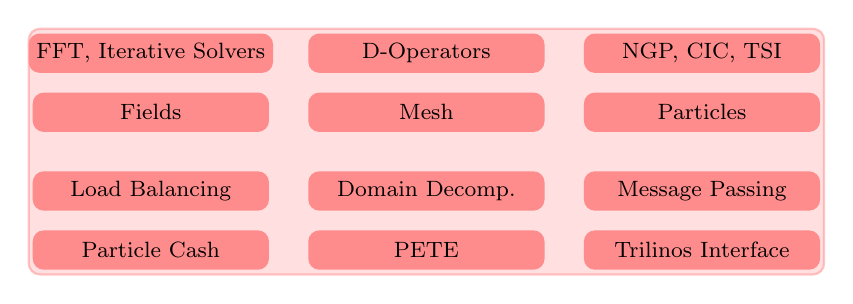
\begin{tikzpicture}[scale=1.0, transform shape]
    \footnotesize
      \begin{scope}[shape=rectangle,rounded corners,minimum width=3.0cm,minimum height=0.5cm,fill=yellow,text centered]
      \draw[rounded corners, draw=red!45, thick, fill=red!25, opacity=0.5, text centered] (-1.55, -0.69) rectangle (8.55,-3.81) 
                node[black, thick, anchor=center, opacity=1.0, font=\Large] at (3.5, -2.25) { };
       \node[fill= red!45] (q_00) at (0,-1) {FFT, Iterative Solvers};
       \node[fill= red!45] (q_01) at (3.5,-1) {D-Operators};
       \node[fill= red!45] (q_02) at (7,-1) {NGP, CIC, TSI};
       \node[fill= red!45] (q_10) at (0,-1.75) {Fields};
       \node[fill= red!45] (q_11) at (3.5,-1.75) {Mesh};
       \node[fill= red!45] (q_12) at (7,-1.75) {Particles};
       \node[fill=red!45] (q_20) at (0,-2.75) {Load Balancing};
       \node[fill=red!45] (q_21) at (3.5,-2.75) {Domain Decomp.};
       \node[fill=red!45] (q_22) at (7,-2.75) {Message Passing};
       \node[fill=red!45] (q_20) at (0,-3.5) {Particle Cash};
       \node[fill=red!45] (q_21) at (3.5,-3.5) {PETE};
       \node[fill=red!45] (q_22) at (7,-3.5) {Trilinos Interface};
      \end{scope}
 \end{tikzpicture}
\end{center}
\caption{Architecture of \ippl}
\label{fig:ippl-noamr}
\end{figure}
Our particle acceleration simulation framework \opal\ is based on
\ippl. The ability to scale to several thousands of cores is shown at
the bottom of Fig.~\ref{fig:xt3opal}.

\noindent \textbf{{Eigenmode calculation}}

The first few eigenfrequencies of the PSI COMET cyclotron could be
computed to high precision with the in-house developed time harmonic
Maxwell solver FemaXX~\cite{geus:02,arge:04}. The large (1.4 million
degrees of freedom) and complex mesh is depicted in
Fig.~\ref{fig:xt3cometfemaxx}, and in addition the parallel speedup
during an eigenmode calculation of PSI's COMET cavities.

\begin{figure}[h]
  \begin{minipage}[b]{\minipagescale\textwidth}
    \includegraphics[angle=\gnuplotrot,scale=1.0]{./figures/Comet.pdf}
    \includegraphics[angle=\gnuplotrot,scale=0.6]{./figures/xt3_comet1.pdf}
  \end{minipage}
  \caption{FemaXX mesh of PSI's COMET cyclotron (left) and speedup
    (right)}
  \label{fig:xt3cometfemaxx}
\end{figure}
Table \ref{tab:cometmeas} shows the excellent agreement between the
calculated and measured eigenfrequencies from PSI's Comet cyclotron. The
number of significant figures in Table \ref{tab:cometmeas} is determined
by the physical boundary conditions of the tuning system and the
accuracy of the measurement process. For the presented system a
resolution of 10 kHz is absolutely sufficient.

\begin{table}[h]\footnotesize
  \caption{Comparison between mode measurements from  PSI's Comet
    cyclotron and the calculated modes}
  \begin{center}  
    \begin{tabular}{lccc} 
      \hline 
      & Measurements [MHz]  & FemaXX \cite{geus:02}  \\
      \hline
      Mode 1 (push/pull)	& 73.18	& 73.18   \\
      Mode 2	&73.41	&73.44 \\
      Mode 3 (pull/pull) &	73.64	&73.69 \\
      Mode 4 &	92.71&	92.46 \\
      \hline
    \end{tabular}
    \label{tab:cometmeas}
  \end{center}
\end{table}


\noindent \textbf{{Space charge calculations at the PSI \hipa\ facility}}

For the quantitative evaluation of the effects of space charge in the
high intensity proton accelerator complex and the SwissFEL, an efficient
three-dimensional particle tracking framework Object Oriented Parallel
Accelerator Library (\opal)~\cite{opal:1} was developed.  Today \opal\
is the key tool to better understand the nonlinear space charge effects
in the present and future particle accelerators at PSI and in several
other laboratories around the world.

Presently, we study different operation scenarios of the PSI HIPA facility,  in the course of the planned high power upgrade and validate
the physical and numerical mode with experiments. In
Fig.~\ref{fig:xt3opal} (top) the beam intensity of the 8 last turns in
the PSI Ring Cyclotron is compared with calculations. A remarkably good
agreement of the turn patterns is observed and demonstrates the
feasibility of precise beam dynamics simulations.  In bottom part of
Fig.~\ref{fig:xt3opal}, the parallel scalability of the code is shown,
which is absolutely essential for solving multi-scale problems, e.g.\ to
track several millions of particles along kilometers of beam path in the
cyclotrons and beam lines.  The data has been computed on the Cray
massive parallel computer of the Swiss National Supercomputing Centre
(CSCS) in Manno in the framework of the PSI-Horizon collaboration
\cite{horpsi}.
\begin{figure}[h]
  \begin{center}
    \includegraphics[width=.49\linewidth]{./figures/rre4v0108log}
    \includegraphics[angle=\gnuplotrot,scale=0.3]{./figures/drift2c1.pdf}
  \end{center}
  \caption{(Top) Comparison of measured density profiles of the last 8
    turns of the PSI ring cyclotron with \opal\ simulations~\cite{bi:1},
    showing a remarkably good agreement.  (Bottom) the parallel
    efficiency of the \opal\ kernel (strong scaling) is shown together
    with the number of particles pushed per time interval. A uniform
    mesh of size $M=1024^3$ and 3D domain decomposition was used.}
  \label{fig:xt3opal}
\end{figure}


\noindent \textbf{{Summary status of research with respect to
    this proposal}}

The examples shown are good illustrations reflecting the strategy to
closely connect theory and practical application in the developed
methods and codes. In the past we have successfully developed methods
and tools to simulate large and complicated accelerator structures.

In the current research proposal we extend our numerical methods towards
a scalable and efficient AMR and in consequence increasing the level of
detail in key areas such as SwissFEL and high power proton accelerator
modeling.


%%%%%%%%%%%%%%%%%%%%%%%%%%%%%%%%%%%%%%%%%%%%%%%%%%%%%%%%%%%%%%%%%%%%%%%

\subsection{Detailed research plan}

Starting point, including problem description, for this research is \cite{adai:10,adai:11} where we
discuss the scalable parallel solution of the Poisson equation within a
Particle-In-Cell (PIC) code for the simulation of electron beams in
particle accelerators of irregular shape.  The problem is discretized by
Finite Differences.  Depending on the treatment of the Dirichlet
boundary the resulting system of equations is symmetric or `mildly'
nonsymmetric positive definite.  In all cases, the system is solved by
the preconditioned conjugate gradient algorithm with smoothed
aggregation (SA) based algebraic multigrid (AMG) preconditioning.  We
investigate variants of the implementation of SA-AMG that lead to
considerable improvements in the execution times.  We demonstrate good
scalability of the solver on distributed memory parallel processor with
up to 2048 processors.  We have a scalable standalone solver based on
\ippl\ and Trilinos available \footnote{The presented solver is also
  available in \opal\ for production.}  which will be used as a basis
for the AMR project.



\subsubsection{Representation of the AMR hierarchy}

The AMR framework will be based on rectangular grids (the building block
of \ippl).  A main part of this work will involve a more detailed
analysis of the pro's and con's of the various approaches used so far.
It appears to us, that neither \textsf{Dendro} nor \textsf{Chombo} can
be used as is for our goals in this project.  In our existing block
structured framework we heavily use Expression Templates \cite{hae2010}
to assure memory efficiency and maximum speed-up.  Not much work has
been carried out to study the application of such advanced software
approaches to complex problems like AMR.  A sketch of the planed
extension to \ippl\ is shown in Fig.~\ref{fig:ipplext}.

\subsubsection{Load balancing}

Load balancing is of course intimately related with the representation
of the AMR hierarchy but also the particles.  Observing the fact, that
in present simulations the particle integration uses between 30\% to
40\% of the total run time, we must consider this as very important.
All types of load balancing involves communication.  We will further
develop a technique of particle overloading introduced
in~\cite{habib2009} within the AMR context.  Experimental features for
particle overloading are already available in our \ippl\ framework,
cf.~Fig.~\ref{fig:ipplext}.  Such techniques can maybe be seen as a way
to overcome the complexity of hybrid or even multi-core architectures.

\subsubsection{Error estimation and grid refinement/coarsening}

In AMR, errors are estimated in each cell.  This is done repeatedly in
an iterative procedure, or every couple of iteration steps in a time
dependent problem.  Cells in which the ``error indicator'' returns a
value above a threshold are marked.  In a framework as \textsf{Chombo}
the marked cells are clustered to form rectangular grids which will be
members of the next finer grid level.  In a framework as \textsf{Dendro}
marked cells are refined, i.e., the octree is locally expanded.  The 2:1
balance constraint enforces refinements of neighboring cells in order to
limit hanging nodes~\cite{sasl:08}.  A similar procedure is needed to
coarsen cells.

There are several possible error indicators of which we mention two.
\begin{itemize}
\item We can check the density gradient of the space charge fields.
  Finite difference approximations of this gradient are cheap to
  compute.   Gradients above a certain tolerance require mesh refining. 
\item Richardson or $\tau$-extrapolation~\cite{tros:00}.  The latter is
  used by P\"oplau \& van Rienen~\cite{pori2008} in their MOEVE code for
  3D space charge calculations with a self-adaptive multigrid technique.
\end{itemize}


\begin{figure}[htb]
  \begin{center}
    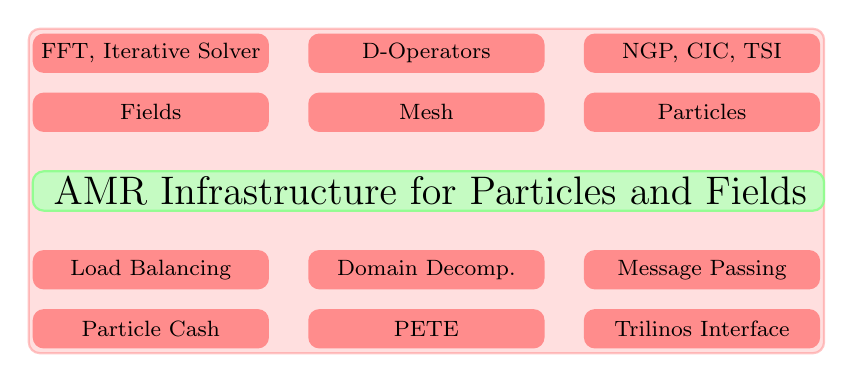
\begin{tikzpicture}[scale=1.0, transform shape]
      \footnotesize
      \begin{scope}[shape=rectangle,rounded corners,minimum
        width=3.0cm,minimum height=0.5cm,fill=yellow,text centered]
        \draw[rounded corners, draw=red!45, thick, fill=red!25,
        opacity=0.5, text centered] (-1.55, -0.69) rectangle
        (8.55,-4.81)
        node[black, thick, anchor=center, opacity=1.0, font=\Large] at
        (3.5, -2.25) { };
        \node[fill= red!45] (q_00) at (0,-1) {FFT, Iterative Solver};
        \node[fill= red!45] (q_01) at (3.5,-1) {D-Operators};
        \node[fill= red!45] (q_02) at (7,-1) {NGP, CIC, TSI};
        \node[fill= red!45] (q_10) at (0,-1.75) {Fields};
        \node[fill= red!45] (q_11) at (3.5,-1.75) {Mesh};
        \node[fill= red!45] (q_12) at (7,-1.75) {Particles};


        \draw[rounded corners, draw=green!45, thick, fill=green!25, opacity=0.9, text centered] (-1.5, -3.0) rectangle (8.55,-2.5) 
        node[black, thick, anchor=center, opacity=1.0, font=\Large] at (3.55, -2.75) {AMR Infrastructure for Particles and Fields };

        % \node[fill= green!45] (q_12) at (0,-2.75) {Particles};


        \node[fill=red!45] (q_20) at (0,-3.75) {Load Balancing};
        \node[fill=red!45] (q_21) at (3.5,-3.75) {Domain Decomp.};
        \node[fill=red!45] (q_22) at (7,-3.75) {Message Passing};
        \node[fill=red!45] (q_20) at (0,-4.5) {Particle Cash};
        \node[fill=red!45] (q_21) at (3.5,-4.5) {PETE};
        \node[fill=red!45] (q_22) at (7,-4.5) {Trilinos Interface};
      \end{scope}
    \end{tikzpicture}
  \end{center}
  \caption{Sketch of \ippl\ with AMR }  \label{fig:ipplext}
\end{figure}

\subsection{Timetable, milestones and deliverables}

The project is planned to last 3 years.  The various phases are
summarized in Tab.~\ref{tbl:time} and detailed information on some of
the activities are given below.

\begin{enumerate}

\item Basic introduction to get the student acquainted with the physics
  of the problem and the state-of-the-art of problem solving strategies
  in the field.

\item A theoretical model and (sequential) prototypical code is
  available.  This code will be used to benchmark the AMR strategy.
  Here, the first interesting research question will be answered: for
  the problems at hand, is it of value to combine a hierarchy of grids
  with an octree-like approach?

\item With the parallel stand-alone solver we benchmark memory and
  parallel efficiency and time to solution on a toy problem set.  We
  also focus on the interoperability with external mesh generation,
  post-processing and efficient handling of input and output.

\item \opal\ is based on \ippl\ and designed using modern software
  engineering approaches such as Design Patterns and Expression
  Templates.  The integration of the AMR capabilities into \opal\ is
  guided by staff scientists and post doctoral researchers within the
  AMAS group, in order to minimize technical overhead for the Ph.D
  student.  The integration will allow us to immediately apply the
  method to challenging problems within the SwissFEL or (in the second
  priority) the PSI proton cyclotron complex.  The second paper to be
  written will focus on the application of AMR to these problems.
\end{enumerate}

We plan to present partial results at international conferences.

\begin{table}[ht]\footnotesize
  \begin{center}  
    \begin{tabular}{lclllll} 
      \hline 
      \bf & \bf Month  & \bf Activity & \bf Milestone  \\
      \hline \\
      % \hline
      1 & 1-5  & Basic introduction to accelerator physics, AMR concepts
      & Ph.D. candidate understands the \\ 
      &       & Understand our existing code base (\ippl\ \& \opal\ )
      & environment and problem to solve\\ 
      &       &                                          & \\
      2 &	4-13  & Developing general AMR strategies  which are
      & Theoretical model and serial prototype   \\ 
      & &  scalable and memory efficient      &   \\
      &       &                                          & \\
      3 &	13-27 & Develop, implement and benchmark        &
      Performance of the AMR solver can be measured\\ 
      &       & the parallel AMR framework based on \ippl     & on a toy
      problem. Writing first paper. \\ 
      &       & 		          	                     & \\
      4 &	27-36 &	Integration of the solver into \opal &Real
      problems can be solved. Writing second paper. \\  
      &       &                   	                     & \\  
      5 &	30-36 &	Writing the thesis                       &
      Ph.D. examination \\ 
      \hline 
    \end{tabular} 
    \caption{Time schedule of the proposed Ph.D. project}
    \label{tbl:time}
  \end{center}
\end{table}


%%%%%%%%%%%%%%%%%%%%%%%%%%%%%%%%%%%%%%%%%%%%%%%%%%%%%%%%%%%%%%%%%%%%%%%

\subsection{Significance of the planned research to the scientific
  community and to eventual potential users}

\label{sec:sign}

A memory efficient and scalable AMR solver for space charge problems is
in general of interest to many people working on challenging problems in
particle accelerator science.  In the primary context that concerns the
SwissFEL project and the upgrade/performance increase of the PSI HIPA
facility, a greater level of detail in simulations is of great
importance.  This is particularly true if it does not come with an
increase of the time to solution.  Such software would, for the first
time, make possible start-to-end simulations with a detailed
characterization of the six-dimensional phase space at every location in
the machine, with required resolution better than $10^{-5} \cdots
10^{-6}$ of the total intensity.

The more abstract question we will address is: What is the most
efficient representation of data in a scalable AMR framework for both
particles and fields.  Future computer systems are anticipated to have
less memory per core.  Hence answers to this question are of utmost
importance.

The scientific consequences will influence research in the areas of
numerical, computational and high performance computing.


%%%%%%%%%%%%%%%%%%%%%%%%%%%%%%%%%%%%%%%%%%%%%%%%%%%%%%%%%%%%%%%%%%%%%%%

\subsection{Significance with respect to scientific, commercial, and
  other application areas}
\label{sec:sign2}
We do not plan to commercialize this research, we plan to put it under a free software license. 


%\nocite{hens:05,cale:05,gbgk:05,vslk:09}
{\small
  \bibliography{amr,citation-aa}
  \bibliographystyle{plain}
}

\end{document}
